\documentclass[draft, 12pt]{article}
\usepackage[english]{babel}
\usepackage[final]{graphicx}
\usepackage{multirow}
\usepackage{color}
\graphicspath{ {figures/} }
\DeclareGraphicsExtensions{.png}

\newcommand{\cc}[1]{\textcolor{red}{#1}}

\title{Seismic parameter estimation and the Canadian crust}
\author{Ben Postlethwaite}

%% ------------------------------------------------------------------------ %%
\begin{document}

\begin{abstract}

\end{abstract}

%% -----------------------------------------------%%
\section{Introduction}

Seismic studies of the Canadian continental crust predominately analyze specific geological features or regions rather than taking a comprehensive and comparative inter-regional analysis. The primary reason for this is the poor resolution afforded by the seismic networks currently and historically deployed across Canada. The Canadian continental landmass is composed of at least fifteen large geological provinces as recognized by the Geological Survey of Canada (GSC). Each of these regions is itself complex and heterogeneous and often larger than most European nations. On top of this there is poor seismic coverage, roughly one seismic station per 25,000 $km^2$. Many of these stations are clustered near areas of geologic interest such as the Cascadia Subduction zone or population and research centres such as Southern Ontario or areas of significant resource interest like the diamondiferous Great Slave Lake area. This leaves vast areas of the Canadian landmass completely unsampled. Despite these limitations, a low resolution comprehensive and comparative study is still feasible for some of the geological regions comprising the Canadian continental crust. Direct comparison between the bulk average seismic properties of geological regions and between aggregated regions and global averages provide some new insight into the crustal composition of the Canadian landmass. The accumulated dataset also affords investigations into variations of bulk crustal parameters such as Poisson's Ratio and crustal thickness with age and tectonic environment as well as some basic statistical data on interesting crustal features.

This paper presents a comparative tour through the dataset accumulated from processing more than a decade worth of data from all available Canadian seismic stations. It begins with a discussion of the raw data itself followed by a review of the receiver function method and a more detailed explanation of the inversion algorithms used to produce the dataset. Three previous publications utilizing similar processing schemes provide unique subsets of data to compare with the values computed in this survey for quality assurance. ...


\subsection{Geological and tectonic summary}


\subsection{Previous geophysical studies}

%% -----------------------------------------------%%
\section{Data and methods}
Our analysis of bulk Canadian continental crust is based on estimates of crustal properties that can be accessed via seismic techniques, namely seismic wave velocities (or velocity ratio) and crustal thickness. This study draws on three sources for these crustal properties. The first and primary source are teleseismic receiver functions (hereafter RFs). The remaining two datasets are Crust 2.0, a widely published statistical average of similar regions with a global two degree resolution and a compilation of pre-processed active source data (Mooney, 2012). Both Crust 2.0 and the active source compilation are used to qualify and compare with the primary dataset.

\subsection{Teleseismic Data Set}
The primary data utilized in this study are computed from teleseismic P-wave seismograms originating from more than 700 earthquake sources. These earthquakes occurred between the years 2000 and 2012 and were recorded on subsets of 343 broadband seismic stations distributed across Canada. Seismic stations are selected from all available regional and national networks including CNSN, Polaris, FedNor and Chasme. Seismograms are included for analysis if they within a 30 to 100$^\circ$ epicentral distance window. Quality control is performed by admitting only those seismograms with high enough signal to noise ratios to permit visual observation of the dominant P-wave energy and with sufficient impulsive first arrivals that allow arrival times to be accurately measured. After selection and filtering more than 80,000 events are available for further processing.

The first stage of processing requires the transformation of teleseismic data into receiver functions. In general terms, this transformation involves deconvolving an approximation of the earthquake source from horizontal recordings of ground motion [Langston, 1979]. The resulting waveforms contain discrete pulses corresponding to the S-wave arrivals scattered from subsurface discontinuities including the base of the crust, or Moho. Confident identification of these peaks to the estimate of crustal parameters, and improved results can be obtained by transforming the seismogram channels into P and S contributions based on a 1-D model of propagation. This procedure is accomplished by first rotating the N and E coordinates into radial and transverse directions and then performing a wave field decomposition using the radial and vertical channels [Bostock, 1998]. The direct arrival of the signal on the resulting P wave component is used as an approximation to the source function as P-wave impulse response for teleseismic P approximates a delta function. This windowed source estimate is deconvolved from the S wave component computed from the wave field decomposition.

We employ $L_2$, multichannel, frequency domain approach to perform the deconvolution which has the advantage of computational efficiency and does not require a priori assumptions about the noise in the data. More specifically, we employ a simultaneous deconvolution of $N$ seismograms sharing a similar slowness to compute a single impulse response or receiver function $r(t)$.

% Deconvolution equations
\begin{equation}
  r(t) = F^{-1} \left[ G(\omega) \right] = F^{-1}
 \left[ \frac {\sum_n^N S_n(\omega)P_n^*(\omega)} {\sum_n^N P_n(\omega)P_n^*(\omega) + \delta} \right ],
\end{equation}

where $F^{-1}$ is the inverse Fourier transform, $S_n$ represents the $n^{th}$ S wave component, $P_n$ is the windowed P wave component, $^*$ denotes the complex conjugate and $\delta$ is the regularization parameter controlling the trade off between model smoothness and data misfit. The parameter $\delta$ is chosen programatically by minimizing the general cross validation function $GCV(\delta)$ which is given by

\begin{equation}
  GCV(\delta) = \frac {\sum_n^N\sum_m^M \left( S_n(\omega_m) - P_n(\omega_m)G(\omega_m) \right)^2 }
                      { \left( NM - \sum_m^M X(\omega_m) \right)^2 },
\end{equation}

where

\begin{equation}
  X(\omega) = \frac {\sum_n^N P_n(\omega)P_n^*(\omega)} {\sum_n^N P_n(\omega)P_n^*(\omega) + \delta},
\end{equation}

and $\omega_m$ is the $m^{th}$ frequency bin in the discrete Fourier transform.

  All resulting receiver functions, $r(t)$, are filtered between 0.04Hz and 3.0Hz.

\subsection{Vp/Vs method} \label{section:VpVsMethod}

\begin{figure}
  \centering
    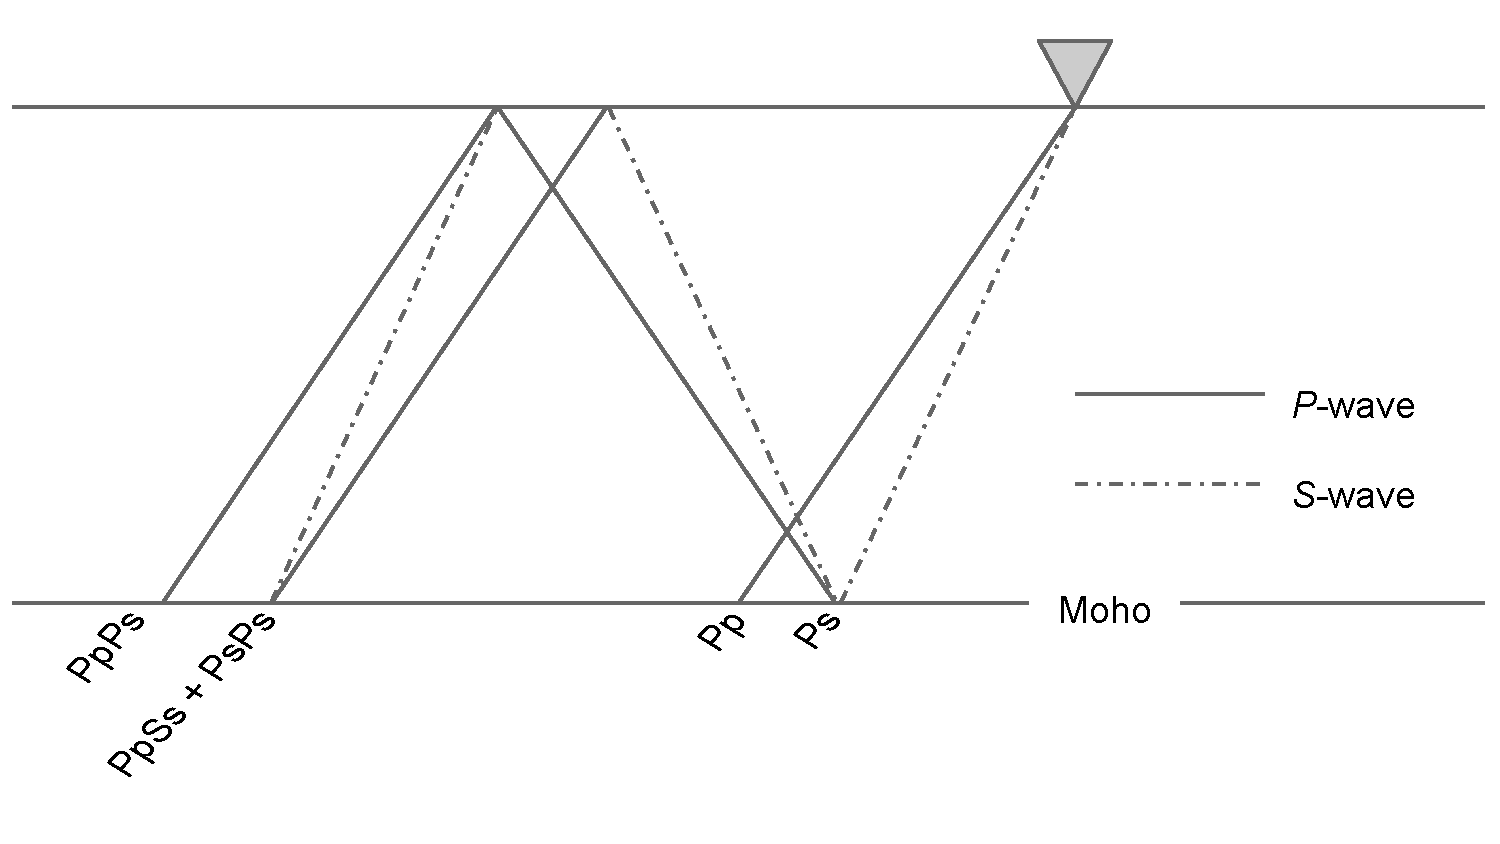
\includegraphics[width=\textwidth]{reflectedPhases}
  \caption{Schematic diagram illustrating geometry of phases for the velocity contrast representing the Moho}
  \label{fig:reflectedPhases}
\end{figure}


A well tested and widely published method for extracting the $\frac{V_P}{V_S}$ ratio $R$ (where $V_P$ is P wave velocity and $V_S$ is S-wave velocity) and crustal thickness (or depth to Moho) $H$, is outlined by Zhu and Kanamori [2000], hereafter ZK. This method takes advantage of the differential arrival times between the S-wave reflected phases $Ps$, $PpPs$, $PsPs$, $PpSs$ and $PsSs$ and the direct P-wave arrival $Pp$ (Fig \ref{fig:reflectedPhases}). Note that $PsPs$ and $PpSs$ are kinematic analogues, such that the energy for these two phases arrive simultaneously for a 1-D model {\it COMMENT: note that the first phase is 2nd order whereas the 2nd is first
order in scattering strength, which is hwy PsPs is not always considered}. For a range of slowness values, $p$, the differential arrival times, $t(p)$, trace moveout curves for each phase arrival given by
ve

% Travel time equations
\begin{equation} \label{eq:tps}
t_{Ps}(p_i)=H \left[ \sqrt{ \left(\frac{R}{V_P}\right)^2 - p_i^2} - \sqrt{\frac{1}{V_P^2} - p_i^2} \right]
\end{equation}

\begin{equation}
t_{Pps}(p_i)=H \left[ \sqrt{ \left(\frac{R}{V_P}\right)^2 - p_i^2} + \sqrt{\frac{1}{V_P^2} - p_i^2} \right]
\end{equation}

\begin{equation}
t_{Pss}(p_i)= 2H  \sqrt{ \left(\frac{R}{V_P}\right)^2 - p_i^2}
\end{equation}

where $p_i$ is the slowness for the $i^{th}$ receiver function. Since strong reflected phases occur at sharp velocity contrasts, the Moho, the boundary targeted by ZK, tends to be well represented on most RF's.

The travel time equations, as employed by ZK, assume a value for crustal P-wave velocity, $V_P$, that in practice will trade-off to some degree with crustal thickness $H$. In our implementation of the ZK approach, each station is assigned a $V_P$ value corrisponding to the Crust 2.0 value for the $2^\circ$ containing cell. In the specific cases where data are being compared to previously published results for quality control, $V_P$  values are chosen to match the values in the published study.

RFs are stacked along trial moveout curves for a range of candidate models of $R$ and $H$ to generate a fitness function $s(H,R)$.  Within the stacking procedure, each phase is assigned a weight to account for a general trend in the quality of the phases, with direct conversion $Ps$ usually characterized by the highest quality signal followed by $PpPs$ and $PpSs$. We chose weights of $w1 = 0.5$, $w2 = 0.3$ , $w3 = -0.2$ for the $Ps$, $PpPs$ and $PpSs$ phases, respectively. A negative weight for the combined $PpSs$ and $PsPs$ phases is required as the polarity of the signal is reversed. Semblance weighting [Eaton, 2006] is employed to reduce the effect of spurious large amplitude noise in the data. The semblance function assigns a weight between zero (incoherent noise) and one (coherent signal). The stacking function is therefore defined as

\begin{equation}  \label{eq:stack}
s(H,R) = \sum_{j=1}^{3} S_j \sum_{i=1}^N w_jr_i(t_j)
\end{equation}

where

\begin{equation}
S_j(H,R) = \frac {\left[ \sum_{i=1}^N r_i(t_j) \right]^2}
                 { \sum_{i=1}^N r_i^2(t_j) }
\end{equation}

is the semblance weight for the $j^{th}$ phase, time $t_j$ is calculated from the corresponding travel time function for a given $H$, $R$ pair as a function of slowness $p_i$ and $N$ is the total number of receiver functions. Multiplying by the semblance weighting sharpens the stacked image, $s(H,R)$, and results in better resolution when discriminating between different models. The function $s(H,R)$ can be thought of as a transformation that maps the $Ps$, $PpPs$ and $PpSs+PsPs$ pulses of the receiver function, $r(t)$, into $R$ and $H$ space as positive bands, via Eq. \ref{eq:stack}. Constructive interference where these bands intersect will produce a maximum in the stacking function. The model, $R$ and $H$, which produce this maximum provides the best estimate for the bulk crustal parameters for a given seismic station.

%% [[\subsection{Full Parameter Method}]]
A limitation of the ZK approach is the requirement for an initial $V_P$ estimate. This can be resolved by computing the stacking function Eq. \ref{eq:stack}, as a function of all three seismic parameters, $s(H,R,V_P)$. Taking advantage of modern multi-core systems with reasonable quantities of data (fifty to a few hundred RFs) and a moderate search space ($n^3$ parameter candidates where $n \approx 150$) the computational time makes this method easily scalable to hundreds of stations. This approach, denoted FG, is analyzed to determine the viability of recovering $V_P$.

The trade-off between $V_P$ and $H$ (and other parameter combinations) and error resulting from data quality are quantified for both the full parameter search and ZK methods by bootstrap resampling [Efron and Tibshirani, 1986]. An estimate for the error is calculated in a bootstrap resampling approach by taking the standard deviation of 1024 parameter estimates each produced with randomly selected RFs, with replacement.

\subsection{Additional data}

We supplement receiver function estimates of crustal properties with data from controlled source experiments collected and compiled from GSC (Geological Survey of Canada) references by Walter Mooney (personal communication, 2012). The active source data provide $V_P$ and a few $V_S$ estimates for hundreds of locations across Canada, many along transects that cross geological provincial boundaries, faults and discontinuities. Some of these data are located within reasonable ($<$100km) proximity to seismic stations used in this study and can be used to compare with the $V_P$ and $V_S$ estimates resulting from the RF full gridsearch.

The Crust 2.0 model [Bassin, 2000] employs many of these same active source data to provide regular, complete coverage across all of Canada. The model includes estimates of $V_P$ and $V_S$ information with depth at
$2^\circ$ resolution in latitude and longitude. In addition to employing local active source data, Crust 2.0 is also constrained by statistically aggregated data from geographically distant but geologically similar regions. It therefore affords a somewhat independent dataset suited for comparison with the crustal estimates calculated in this study.

%% -----------------------------------------------%%
\section{Results}

\subsection{Comparisons}

Several published regional studies utilizing the methods outlined in section \ref{section:VpVsMethod}, ZK + semblance weighting, provide parameter estimates for $R$ and $H$ for regionally grouped subsets of Canadian seismic stations. Comparisons between estimates for particular seismic stations are made for those values which have a corresponding standard error in $R$ of less than 0.06. This error value best partitions the data between those receiver function stacks with visually recognizable energy along phase moveout curves from those where lack of data or poor quality make these moveout curves difficult to resolve. For each study under comparison, data is reprocessed to use the $V_P$ chosen by the study authors and both correlation and mean difference are calculated (Table \ref{table:comparison}).

\begin{table}
  \begin{tabular}{ l l l l l l }
    \cline{3-6}
    & & \multicolumn{2}{ c }{Correlation} & \multicolumn{2}{ c }{Mean Difference} \\
    \hline
    Study Authors & Num. of Stns & $H$ & $R$ & $H$(km) & $R$ \\
    \hline
    Thompson et. al. (2010)   & 27 & 0.97 & 0.49 & 3.36 & 0.024 \\
    Eaton et. al. (2006)      & 26 & 0.90 & 0.61 & 2.65 & 0.04  \\
    Darbyshire et. al. (2007) & 10 & 0.95 & 0.43 & 4.16 & 0.39  \\
    \hline
  \end{tabular}
  \caption{Comparison of $R$ and $H$ estimates with three published studies}
\label{table:comparison}

\end{table}

All three studies provide $H$ estimates that correlate strongly with the computed crustal thickness parameters. [[maximum mean difference, students ttest ? what would be a good stat for actual dataset difference? ]]. The correlation between the seismic velocity ratio is lower, though due to the lower resolution in $R$ this result is not unexpected. Overall there is good correlation between the estimates from the three studies and the computed estimates.

\subsection{Full Parameter Search Analysis}
Comparing the ZK approach with the full parameter search (Table \ref{table:ZKvsFG}) we see that the velocity ratio $R$ has a correlation between the two datasets of 0.76 while $H$ has a correlation of only 0.51. Since $t_{Ps}$ represents the differential travel time between the S and P wave, the dependence of $H$ on $V_P$ is weak. This means that for a given uncertainty in the three dimensional stack $s(H,R,V_P)$, the gradient in the stack-space will be lowest along the kinematic curve in the $H$ and $V_P$ axis (Figure \ref{fig:HVp_ULM}). This conveys the inherent trade-off in resolution between $H$ and $V_P$ and contributes to the low correlation between the two methods. Parity between the ZK and FG methods can be regained by dividing out $V_P$ from $H$. The trade-off between the other parameters is lower, owing to greater dependence between the parameters in the travel time equations (Figures \ref{fig:HR_ULM}-\ref{fig:RVp_ULM}.

For all but the cleanest stations, the trade-off between $H$ and $V_P$ makes the recoverability of $V_P$ unfeasible using the FG approach. A comparison between two stations, ULM, the station with the highest quality RFs, and DORN, a station exhibiting less resolution in the reflected phases, illustrates this challenge. The horizontally stacked RFs for both stations are ordered by increasing slowness and are shown in figures \ref{fig:RF_ULM} and \ref{fig:RF_DORN}. Cross sections of the three dimensional stack are given for ULM and DORN in figures \ref{fig:HR_ULM}-\ref{fig:HVp_ULM}) and figures \ref{fig:HR_DORN}-\ref{fig:HVp_DORN}. The lower resolution conveyed in the $H$ and $V_P$ cross section for DORN translates into a bootstrap error of $V_P +/- 0.64 km/s$. The station ULM, with cleaner data has a lower absolute trade-off between $H$ and $V_P$ as indicated by the corrisponding cross section and the lower bootstrap error of $V_P +/- 0.16 km/s$.

\begin{table}
  \begin{tabular}{ l l }
    \hline
    Parameter & correlation coeff \\
    \hline
    $R$ (km) &  0.76 \\
    $H$      &  0.51 \\
    $H/V_P$  &  0.96 \\
    \hline
  \end{tabular}
  \caption{Correlation between parameters computed from ZK + semblance and full parameter search methods}
\label{table:ZKvsFG}

\end{table}


\begin{figure}
  \centering
  \includegraphics[width=\textwidth]{RF_ULM}
  \caption{}
  \label{fig:RF_ULM}
\end{figure}

\begin{figure}
  \centering
  \includegraphics[width=\textwidth]{stackHR_ULM}
  \caption{}
  \label{fig:HR_ULM}
\end{figure}

\begin{figure}
  \centering
  \includegraphics[width=\textwidth]{stackRVp_ULM}
  \caption{}
  \label{fig:RVp_ULM}
\end{figure}

\begin{figure}
  \centering
  \includegraphics[width=\textwidth]{stackHVp_ULM}
  \caption{}
  \label{fig:HVp_ULM}
\end{figure}

\begin{figure}
  \centering
  \includegraphics[width=\textwidth]{RF_DORN}
  \caption{}
  \label{fig:RF_DORN}
\end{figure}


\begin{figure}
  \centering
  \includegraphics[width=\textwidth]{stackHR_DORN}
  \caption{}
  \label{fig:HR_DORN}
\end{figure}

\begin{figure}
  \centering
  \includegraphics[width=\textwidth]{stackRVp_DORN}
  \caption{}
  \label{fig:RVp_DORN}
\end{figure}

\begin{figure}
  \centering
  \includegraphics[width=\textwidth]{stackHVp_DORN}
  \caption{}
  \label{fig:HVp_DORN}
\end{figure}


\subsection{Regional Bulk Crustal Parameters}
Parameter estimates for stations assigned less than a 0.6 bootstrap error in the velocity ratio, $R$, are grouped regionally and analyzed. To compensate for the uneven geographic distribution of seismic stations, weights are applied to all crustal parameter estimates before averaging over a given region. Weights are calculated by first projecting station locations onto the 2D plane using the Albers equal-area conic projection. A Voronoi diagram is then calculated using all projected station locations. The ratio between the Voronoi cell surface encompassing each station and the total area of the convex hull bounding region is computed and used as the weighting value.

\begin{table}
  \begin{tabular}{ l l l l l l }
    \cline{2-6}
    & \multicolumn{2}{ c }{ZK + semblance} & \multicolumn{2}{ c }{Crust 2.0} & \multicolumn{1}{ c }{Active Source} \\
    \hline
    Region & $R$ & $H [km]$ & $R$ & $H [km]$ & $V_P [km/s]$ \\
    \hline
    Canada     & 37.0 & 1.75 & 38.2 & 1.77 & 6.33\\
    Shield     & 39.2 & 1.74 & 38.8 & 1.77 & 6.42\\
    Slave      & 38.2 & 1.74 & 37.0 & 1.76 & 6.44\\
    Churchill  & 38.9 & 1.73 & 37.8 & 1.77 & 6.39\\
    Superior   & 39.7 & 1.74 & 39.1 & 1.76 & 6.44\\
    Grenville  & 41.7 & 1.78 & 40.5 & 1.78 & 6.48\\
    \hline
  \end{tabular}
  \caption{Comparison of $R$ and $H$ estimates with three published studies}
\label{table:regionParameters}

\end{table}

Moving South and East from the Churchill through the Superior and the Grenville there is an increase in the ZK + semblance computed seismic velocity ratio as well as crustal thickness. The weighted $R$ average is 1.73 in the Churchill Province increasing slightly to 1.74 in the Superior and jumping to 1.78 in the Grenville. Similarly the weighted average Moho depth increases from 38.9 km in the Churchill to 39.7 in the Superior and 41.7km in the Grenville. The Southeastern trend towards increasing values is also seen in the weighted averaged active source $V_P$ data.  Generally the Crust 2.0 values show a slightly thinner crust though the southward thickening trend is noticeable. The trend in the seismic velocity data is not as apparent in the Crust 2.0 data.

\subsection{Conrad Discontinuity}
Results and figures showing statistics regarding depth of crustal reflectors.
[[ Idea: Statistical test of distributions? How much confidence in a range of modes n = 1->5
   Winning number of modes - partition the dataset for those stations with those modes
   map spatially and see if it is a geographic density bias / trend ]]


\begin{figure}
  \centering
  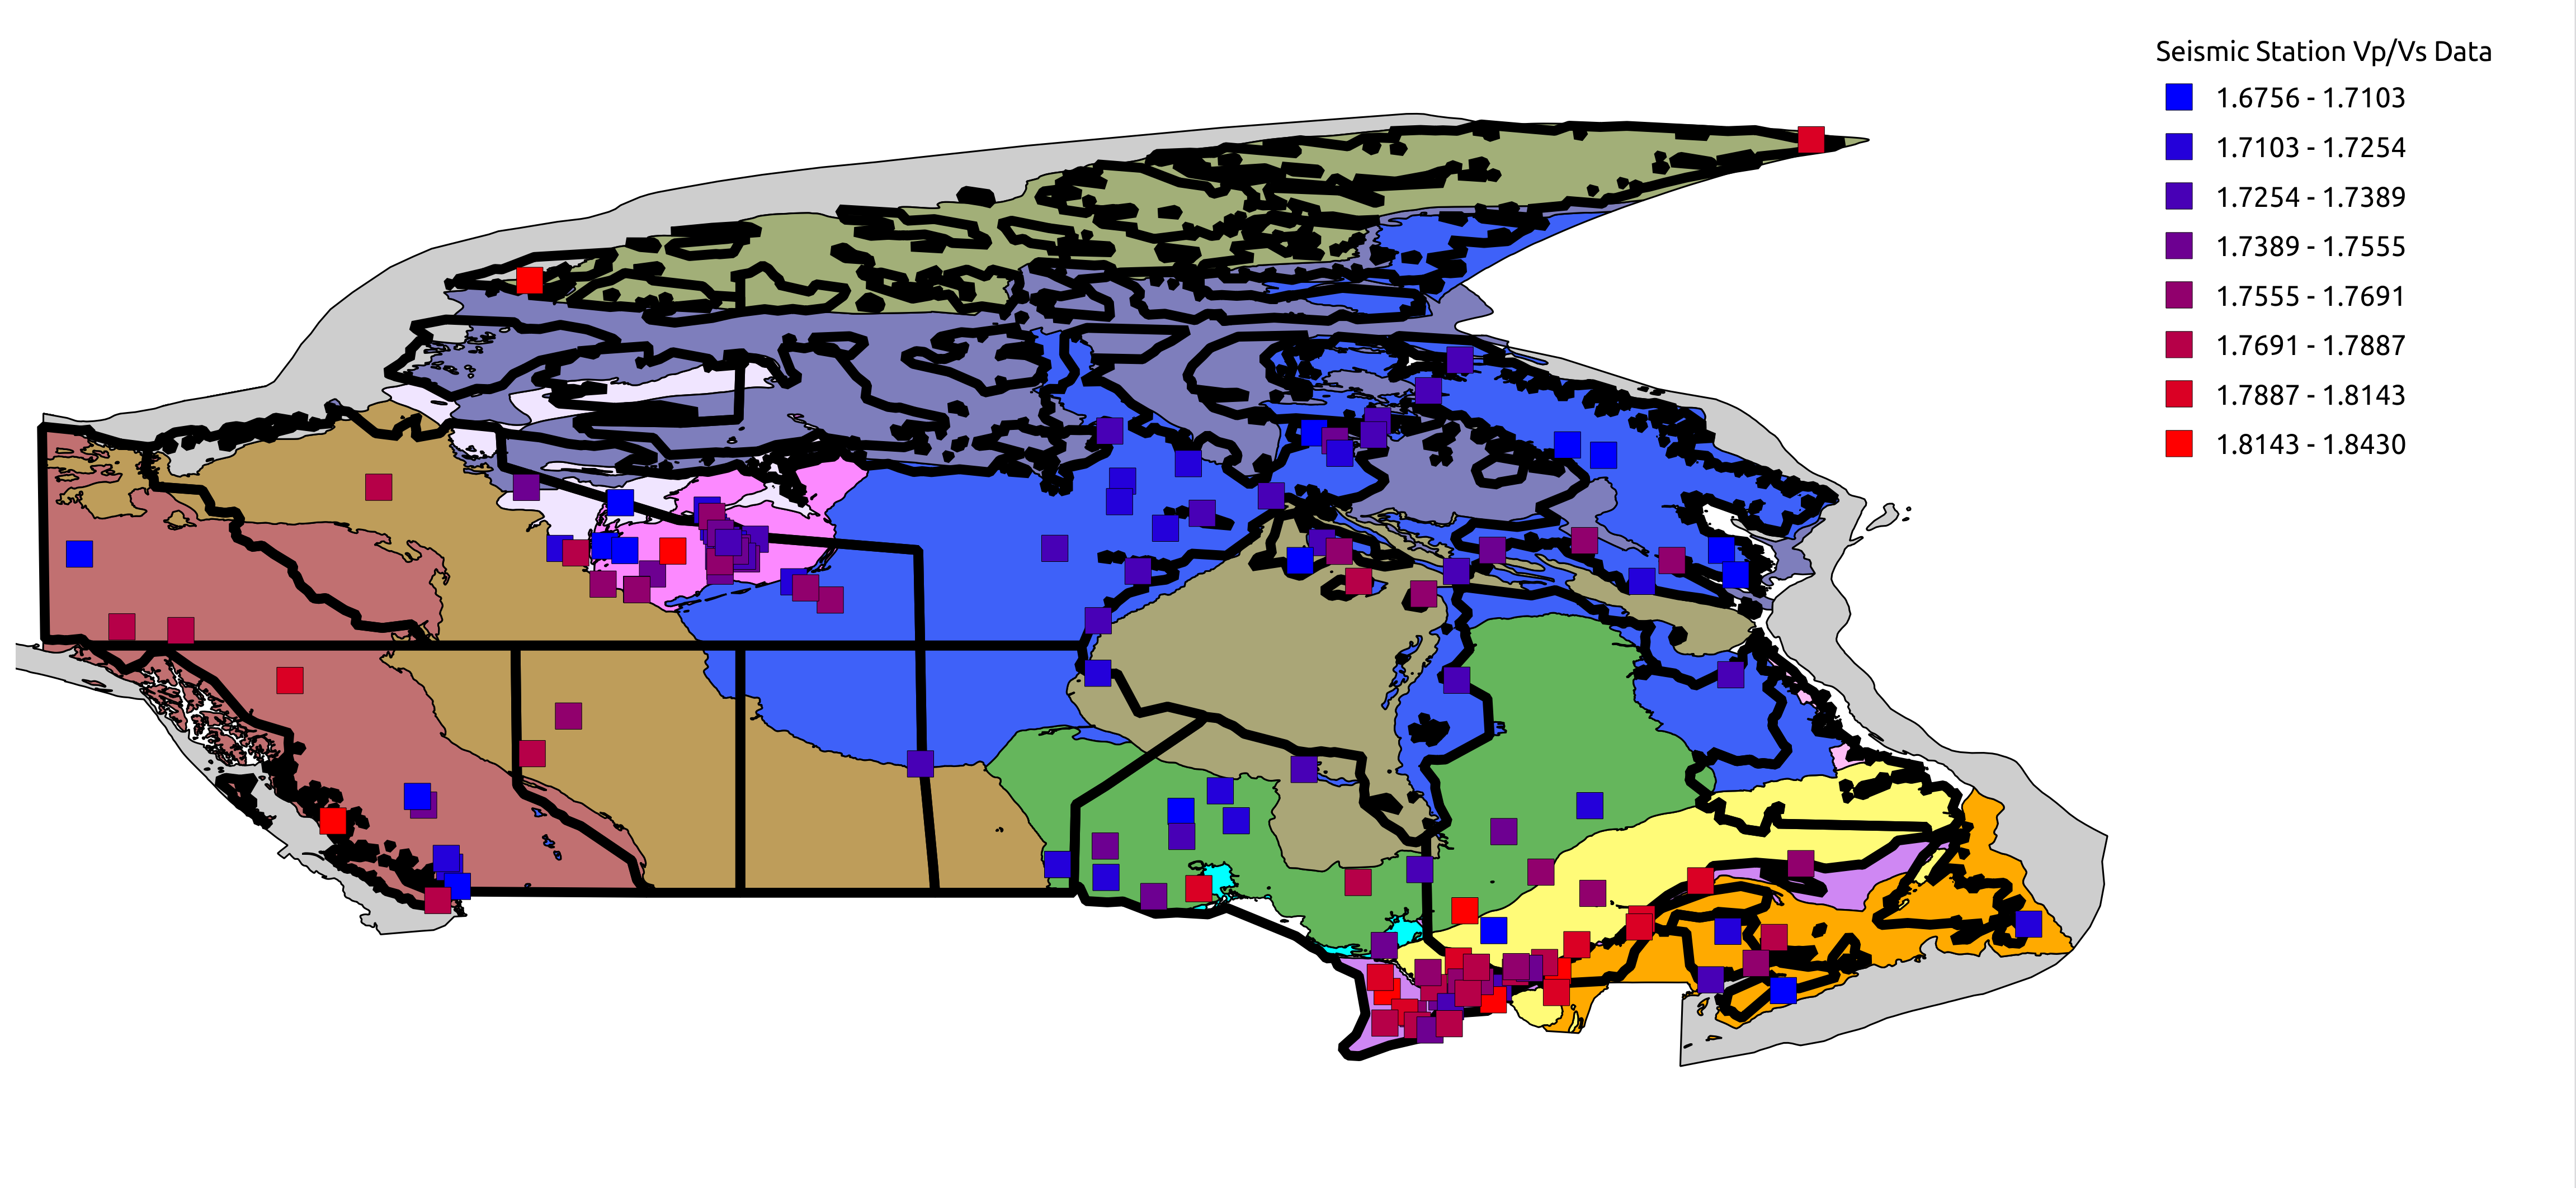
\includegraphics[width=\textwidth]{VpVsMap}
  \caption{}
  \label{fig:VpVsMap}
\end{figure}

\begin{figure}
  \centering
  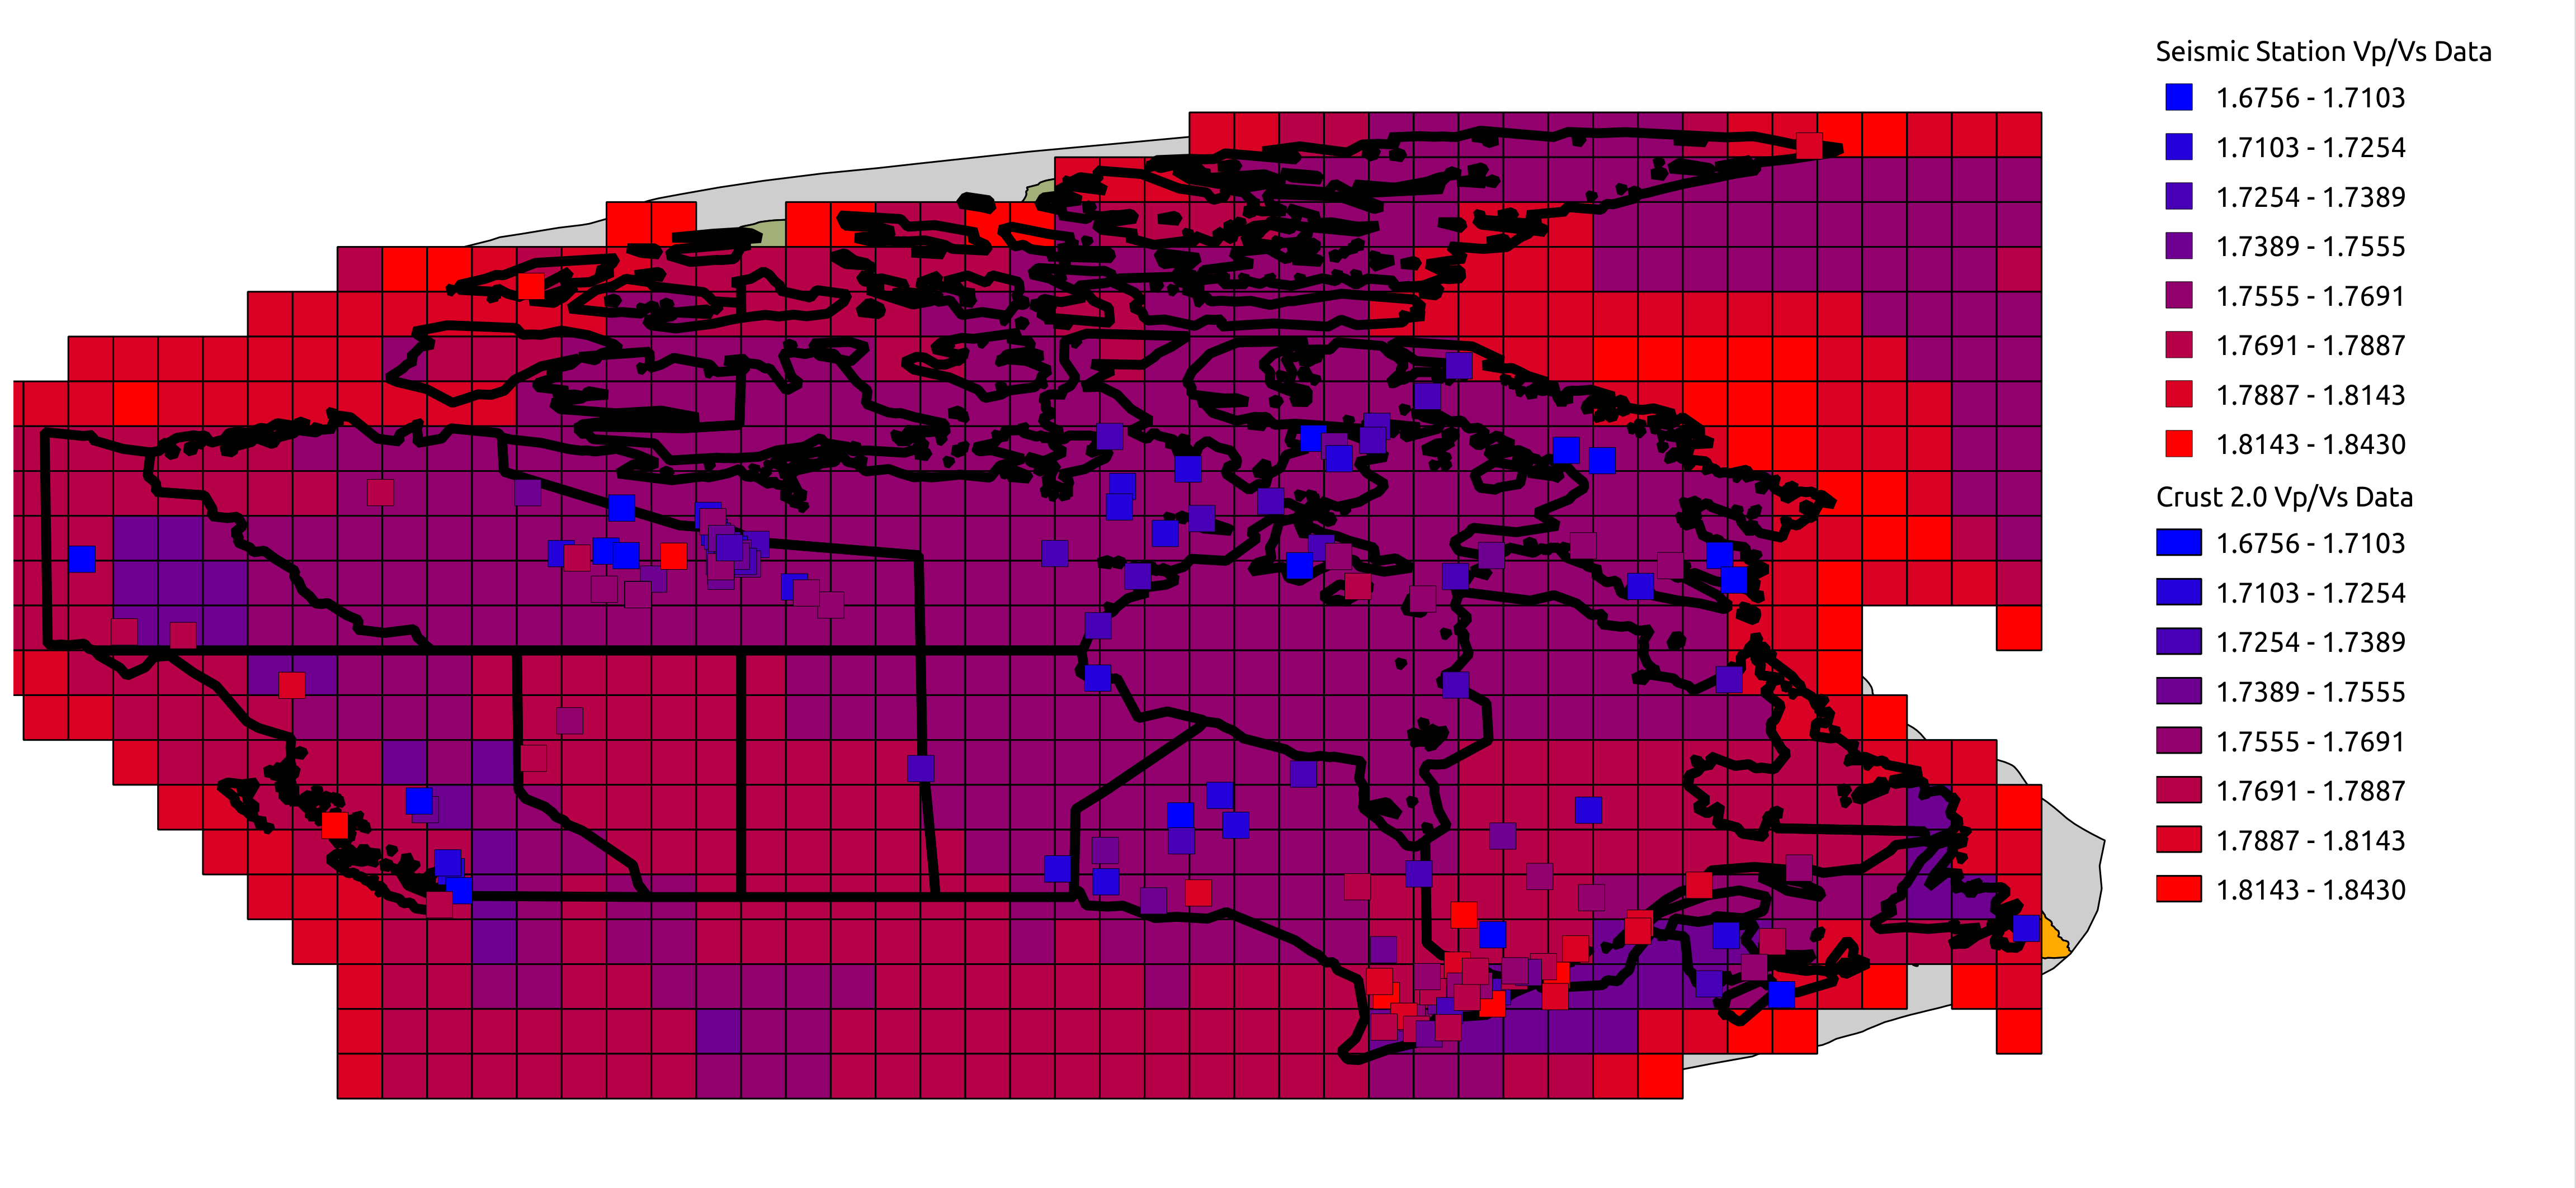
\includegraphics[width=\textwidth]{VpVsMapCrust}
  \caption{}
  \label{fig:VpVsMapCrust}
\end{figure}


%% -----------------------------------------------%%
\section{Discussion}
\subsection{Canada}

  - Comparison Discussion
    - Crustal Thickness
      - Very good correlation in thickness estimates with all three datasets.
    - Vp/Vs
      - Lower correlation with the Vp/Vs values.
        - Expect lower correlation with Vp/Vs since the travel time equations are
          less sensitive to seismic velocities than they are to crustal thickness.
          This means that there will be more uncertainty during the parameter
          search for Vp/Vs and hence higher degree of relative error.
        - ??? Utilizing different sources, applying different deconvolution and
          filtering techniques will therefore have a greater impact on the
          uncertainty of picking Vp/Vs than that of crustal thickness H. ???

   - Explanation of results
    - Canada H and Vp/Vs
      - Lith5.0 (Perry, 2002) estimates for Canadian crustal averages is 38 km. The Crust
        2.0 average is 38km as well, however this is expected since Crust2.0 data for
        Canada is based on the same data as that of Lith5.0
      - ??? Make some comparison to global average ???


%% -----------------------------------------------%%
\section{Conclusions}
Conclusions here

%% ------------------------------------------------------------------------ %%


\begin{bibliography}
Bassin, C., G. Laske, G. Masters (2000), The Current Limits of Resolution for Surface Wave Tomography in North America, EOS Trans AGU, 81.

Bostock, M. G. (1998), Mantle stratigraphy and the evolution of the Slave province, J. Geophys. Res., 103, 21,183-21,200.

Bostock, M. G., M. R. Kumar (2010), Bias in seismic estimates of crustal properties, J. Geophys. Int., 182, 403-407.

Christensen, N. I. (1996), Poisson's ratio and crustal seismology, J. Geophys. Res., 101, 3139–3156.

Darbyshire, F. A., D. W. Eaton, A. W. Frederiksen, E. Leila (2006), New insights into the lithosphere beneath the Superior Province from Rayleigh wave dispersion and receiver function analysis, J. Geophys. Int., 169, 1043-1068.

Durrheim, R. J., W. D. Mooney (1991), Archean and Proterozoic crustal evolution, Geology, 19, 606-609.

Eaton, D. W., S. Dineva, R. Mereu (2005), Crustal thickness and Vp/Vs variations in the Grenville orogen (Ontario, Canada) from analysis of teleseismic receiver functions, Tectonophysics, 420, 223-238.

Efron, B., R. Tibshirani (1986), Bootstrap Methods for Standard Errors, Confidence Intervals, and Other Measures of Statistical Accuracy, Statistical Science, 1, 54-75.

Golub, G. H., M. Heath, G. Wahba (1979), Generalized cross-validation as a method for choosing a good ridge parameter, Technometrics, 21, 215-223.
Mooney, W. D. (2012), Personal communication. Compiled GSC active source data for the Canada.

Langston, C. A. (1979), Structure under Mount Rainier, Washington, inferred from teleseismic body waves, J. Geophys. Res., 84(B9), 4749–4762, doi:10.1029/JB084iB09p04749.

Perry, H. K. C., D. W. S. Eaton, A. M. Forte (2002) LITH5.0: a revised crustal model for Canada based on Lithoprobe results,  J. Geophys. Int., 150, 285-294.

Thompson, D. A., I. D. Bastow, G. Helffrich, J.-M. Kendall, J. Wookey, D. B. Snyder, D. W. Eaton (2010), Precambrian crustal evolution: Seismic constraints from the Canadian Shield, Earth and Planetary Science Letters, 297, 655–666.

Zhu, L., H. Kanamori (2000), Moho depth variation in Southern California from teleseismic receiver functions, J. Geophys. Res., 105, 2969-2980.

Zandt, G., C. J. Ammon (1995), Continental crust composition constrained by measurements of crustal Poisson's ratio, Nature, 374, 152-154.

\end{bibliography}


\end{document}

%% ------------------------------------------------------------------------ %%

